\documentclass{article}

\usepackage{graphicx}
\usepackage{tikz}
\usepackage{tikzsymbols}
\usetikzlibrary{calc,patterns,shapes.geometric}
\pagestyle{empty}
\usepackage[margin=0pt]{geometry}
\geometry{papersize={14in,12in}}

\def\centerarc[#1](#2)(#3:#4:#5){\draw[#1] ($(#2)+({#5*cos(#3)},{#5*sin(#3)})$) arc (#3:#4:#5);}

\begin{document}
	\begin{figure}
		\centering
		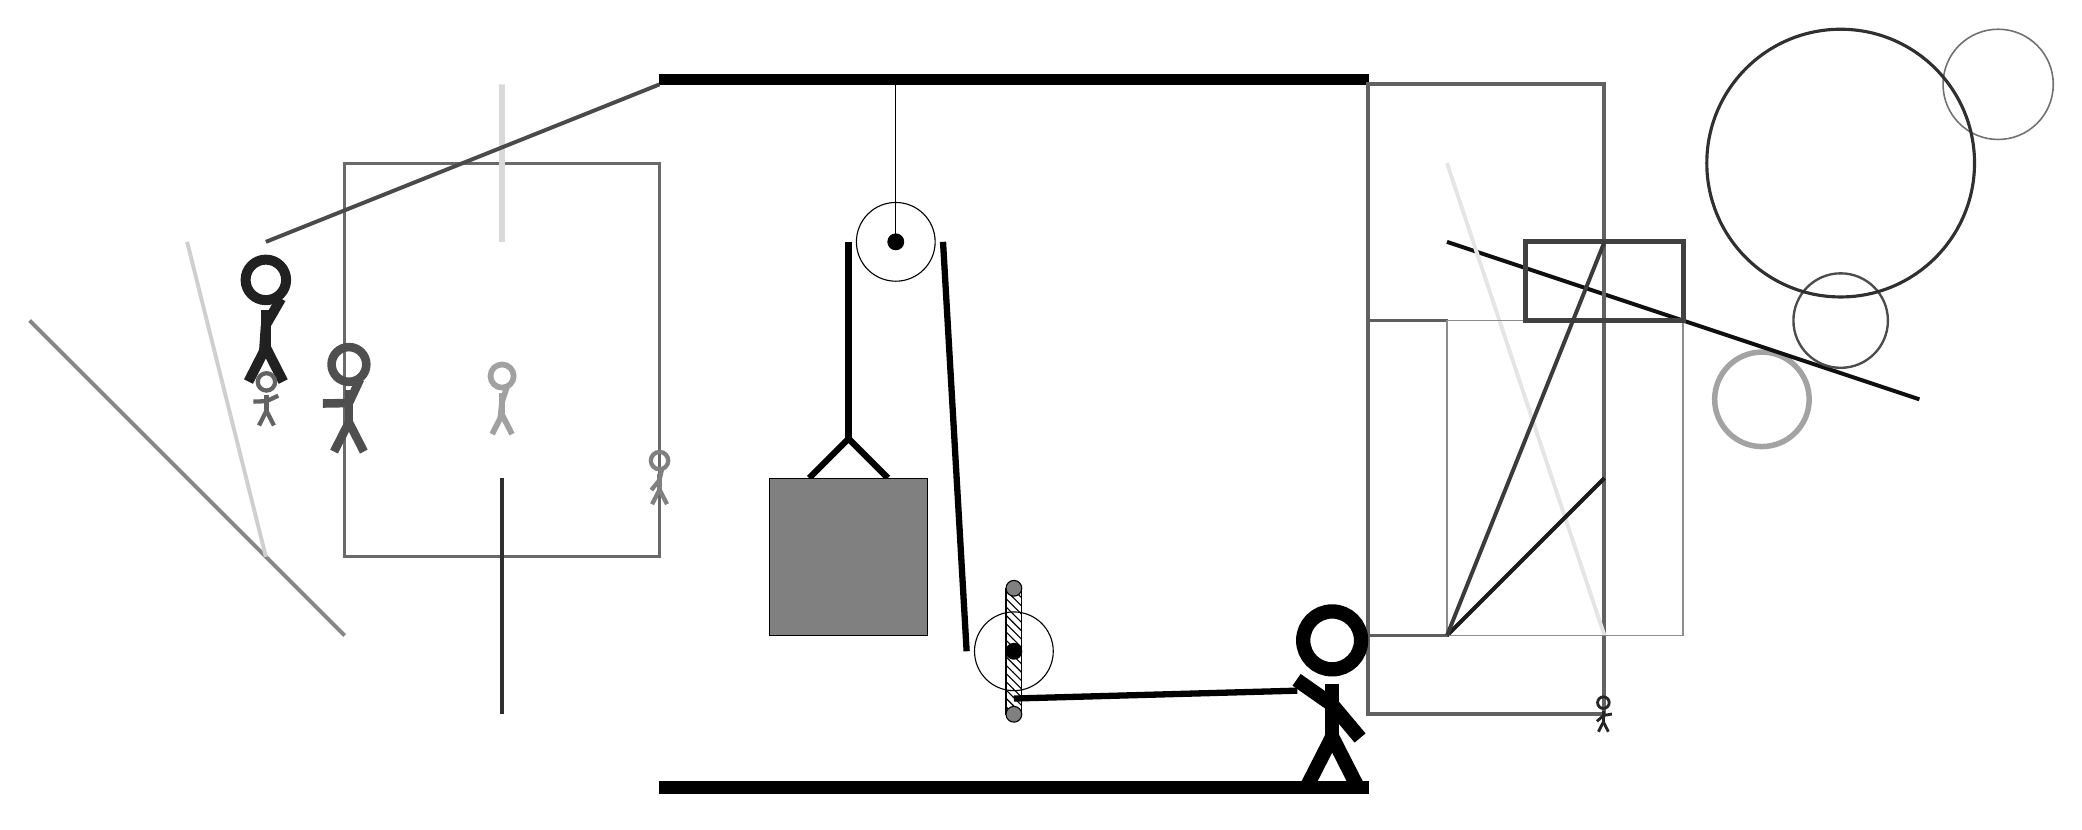
\begin{tikzpicture}
			%%%%% START %%%%%
			
			\draw[fill=black] (-2, 9) rectangle (7, 9.125);
			
			\draw (1, 7) circle (0.5);
			\draw[fill=black] (1, 7) circle (0.1);
			\draw (1, 9) -- (1, 7);
			
			\draw[fill=white](2.5, 1.8) circle (0.5);
			\draw[fill=black] (2.5, 1.8) circle (0.1);
			\draw[pattern=north west lines, pattern color=black] (2.4, 2.6) rectangle (2.6, 1.0);
			\draw[fill=black!50] (2.5, 2.6) circle (0.1);
			\draw[fill=black!50] (2.5, 1.0) circle (0.1);
			
			\draw[line width=0.8mm] (-0.1, 4.0) -- (0.4, 4.5) -- (0.9, 4.0);
			\draw[fill=black!50] (-0.6, 4.0) rectangle (1.4, 2.0);
			
			\draw [line width=0.7mm, color=black!36](12, 5) circle (0.6);
			
			\draw[line width=0.4mm, color=black!59] (-2, 3) rectangle (-6, 8);
			\draw[line width=0.5mm, color=black!94](8, 7) -- (14, 5);
			\draw[line width=0.5mm, color=black!62] (7, 9) rectangle (10, 1);
			\draw[line width=0.5mm, color=black!10](10, 2) -- (8, 8);
			
			\draw [line width=0.2mm, color=black!56](15, 9) circle (0.7);
			\node[line width=0.6mm, color=black!50] at (-2, 4) {\Strichmaxerl[3][51][77]};
			\node[line width=0.7mm, color=black!85] at (10, 1) {\Strichmaxerl[2][42][10]};
			\draw[line width=0.3mm, color=black!63] (7, 2) rectangle (8, 6);
			\node[line width=0.5mm, color=black!87] at (-7, 6) {\Strichmaxerl[7][86][60]};
			\draw[line width=0.5mm, color=black!89](10, 4) -- (8, 2);
			\draw[line width=0.5mm, color=black!47](-6, 2) -- (-10, 6);
			\draw[line width=0.2mm, color=black!45] (8, 2) rectangle (11, 6);
			
			\draw [line width=0.3mm, color=black!70](13, 6) circle (0.6);
			\node[line width=0.3mm, color=black!61] at (-7, 5) {\Strichmaxerl[3][2][25]};
			\draw[line width=0.5mm, color=black!82](-4, 1) -- (-4, 4);
			
			\draw[line width=0.7mm, color=black!15] (-4, 9) rectangle (-4, 7);
			\draw [line width=0.4mm, color=black!81](13, 8) circle (1.7);
			\draw[line width=0.6mm, color=black!75] (9, 6) rectangle (11, 7);
			
			\node[line width=0.5mm, color=black!69] at (-6, 5) {\Strichmaxerl[6][1][65]};
			\draw[line width=0.5mm, color=black!77](10, 7) -- (8, 2);
			\draw[line width=0.5mm, color=black!71](-2, 9) -- (-7, 7);
			\node[line width=0.7mm, color=black!37] at (-4, 5) {\Strichmaxerl[4][84][72]};
			\draw[line width=0.5mm, color=black!19](-7, 3) -- (-8, 7);
			
			\draw[line width=0.8mm] (0.4, 7) -- (0.4, 4.5);
			\centerarc[line width=0.8mm](1, 7)(0:180:0.6);
			\draw[line width=0.8mm](1.6, 7) -- (1.9, 1.8);
			\centerarc[line width=0.8mm](2.5, 1.8)(180:270:0.6);
			\draw[line width=0.8mm](2.5, 1.2) -- (6.1, 1.3);
			
			\node at (6.5, 1.2) {\Strichmaxerl[10][-35][-50]};
			
			\draw[fill=black] (-2, 0) rectangle (7, 0.15);
			
			%%%%% END %%%%%
		\end{tikzpicture}
	\end{figure}	
\end{document}